\chapter{Higgs boson at the LHC: Phenomenology}
\label{sec:LHC_Pheno}
\chaptermark{Higgs boson at the LHC: Phenomenology}


In this section we discuss specific phenomenological details that are studied for this thesis. First, we discuss the different modes of producing a Higgs boson at the LHC, and different features of these different production modes. Next, we will present the decay of a Higgs boson into two Z bosons and subsequently four leptons. Using this information we will present the implications of off resonance production and decay on the Higgs boson lifetime. Finally, we will discuss the spin and parity of a single-produced resonance and how we can use these relations to characterize a new particle found at the LHC.

\section{Higgs boson production at LHC}
\label{sec:Higgs_Production_Pheno}

In proton-proton collisions a SM Higgs boson can be produced through the coupling of a Higgs boson to either bosons or fermions. Each of these two categories of Higgs boson production will be dominated by specific production modes. Fermionic production of a Higgs boson can happen either through \textit{gluon-gluon fusion} $gg \to H$ (ggH) and much less frequently through production in \textit{association with two top quarks} $gg \to H + t\bar{t}$ ($t\bar{t}H$). Bosonic production of a Higgs boson can occur through \textit{vector boson fusion} (VBF), where two quarks radiate vector bosons which produce the boson in association with two quark jets $qq \to H + 2\text{jets}$ or through production \textit{associated with a vector boson} $qq \to H + W/Z$ (VH).

The cross sections of these different production mechanisms as a function of the Higgs boson mass at the LHC are shown in figure \ref{fig:LHC_Hxsec} for the two center of mass energies used in this thesis; $\sqrt{s} = \unit{7}{\TeV}$ and $\sqrt{s} = \unit{8}{\TeV}$ \cite{Dittmaier:2011ti, Dittmaier:2012vm}. Notable features of these cross sections are the order of magnitude difference between gluon-gluon fusion and the bosonic production modes which are all much larger than the $H + t\bar{t}$ production. Additionally, one can see the boost in the gluon-gluon fusion production at $2m_{t}$, which corresponds to the top quark in the production loop going becoming on shell (explained in more detail below).

\begin{figure}
\begin{center}
\includegraphics[width=0.46\linewidth]{{LHC_Pheno/Higgs_XS_7TeV}.pdf}
\includegraphics[width=0.455\linewidth]{{LHC_Pheno/Higgs_XS_8TeV_lx}.pdf}
\caption[Standard Model Higgs boson production cross sections and relative uncertainties at $\sqrt{s} = \unit{7}{\TeV}$ and $\sqrt{s} = \unit{8}{\TeV}$. From top to bottom these are $pp \to H$, blue, $pp \to H + 2\text{jets}$, red, $pp \to H + W$, green, $pp \to H + Z$, grey, $pp \to H + t\bar{t}$, purple.]{Standard Model Higgs boson production cross sections and relative uncertainties at $\sqrt{s} = \unit{7}{\TeV}$ and $\sqrt{s} = \unit{8}{\TeV}$. From top to bottom these are $pp \to H$, blue, $pp \to H + 2\text{jets}$, red, $pp \to H + W$, green, $pp \to H + Z$, grey, $pp \to H + t\bar{t}$, purple \cite{Dittmaier:2011ti, Dittmaier:2012vm}.}
\label{fig:LHC_Hxsec}
\end{center}
\end{figure}

The main production mechanism at the LHC is gluon-gluon fusion. The Feynman diagram for this process is shown in figure \ref{fig:ggH_Feyn}. While the Higgs boson does not couple directly to gluons (because they are massless) this mode of production relies on the Higgs boson coupling to fermions generated by the incoming gluons. Because the coupling of the Higgs boson is proportional to the mass of the fermion the dominant contribution is the Higgs boson -- top coupling. This leads to a boost in the cross section when the mass of the Higgs boson is twice the top mass because the top in the loop shown is no longer virtual. For the entire mass range that is considered in this analysis this is the most common way to produce a Higgs boson at the LHC.

\begin{figure}
\begin{center}
\unitlength=1mm
\begin{fmffile}{ggH_Feyn}

\begin{fmfgraph*}(40,30) 
  \fmfleft{i1,i2} \fmfright{sp1}
  \fmf{gluon,label=$g$}{i1,v1} 
  \fmf{gluon,label=$g$}{i2,v2}
  \fmf{fermion}{v1,v2,v3,v1}
  \fmffixed{(0,.6h)}{v1,v2}
  \fmf{dashes,label=$H$}{v3,sp1}
\end{fmfgraph*}

\end{fmffile}
\end{center}
\caption[Feynman diagram depicting Higgs boson production through gluon-gluon fusion $gg \to H$. The fermion loop is dominated by top quarks, however all quarks contribute according to their masses.]{Feynman diagram depicting Higgs boson production through gluon-gluon fusion $gg \to H$. The fermion loop is dominated by top quarks, however all quarks contribute according to their masses.}
\label{fig:ggH_Feyn}
\end{figure}

The second most likely way to produce a Higgs boson at the LHC is through vector boson fusion. To produce a Higgs boson this way two quarks each radiate a W or Z boson which fuse into the Higgs boson. This production mode relies on the Higgs boson coupling to the vector bosons, making it distinct compared to gluon-gluon fusion. the distinguishing feature of this production mode is the presence of two quark jets in the final state in addition to the Higgs boson. These jets contain information about the Higgs boson and can be exploited to refine searches and study the properties of a new particle. The Feynman diagram for this process is shown in figure \ref{fig:qqH_Feyn}.

\begin{figure}
\begin{center}
\unitlength=1mm
\begin{fmffile}{qqH_Feyn}

\begin{fmfgraph*}(40,30) 
  \fmfleft{i1,i2} \fmfright{sp1,sp2,sp3}
  \fmf{fermion,label=$q$}{i1,v1,sp1} 
  \fmf{fermion,label=$q$}{i2,v2,sp3}
  \fmf{boson,label=$W/Z$,label.side=left}{v1,v3}
  \fmf{boson}{v3,v2}
  \fmffixed{(0,.3h)}{v1,v3}
  \fmffixed{(0,.3h)}{v3,v2}
  \fmf{dashes,label=$H$}{v3,sp2}
\end{fmfgraph*}

\end{fmffile}
\end{center}
\caption[Feynman diagram depicting Higgs boson production through vector boson fusion $qq \to H + 2\text{jets}$.]{Feynman diagram depicting Higgs boson production through vector boson fusion $qq \to H + 2\text{jets}$.}
\label{fig:qqH_Feyn}
\end{figure}

Sub-dominant to these two production modes are processes that produce a Higgs boson in association with vector bosons or top quarks. This thesis does not tune the analysis to separate these modes from the dominant ones, instead they are grouped with the dominant modes by how the Higgs boson couples to the other standard model particles. VBF is grouped with VH because the Higgs boson is produced through a coupling to vector bosons while $t\bar{t}H$ is grouped with ggH because it relies on the Higgs boson coupling to fermions.

Producing the Higgs boson in association with a W or Z boson is conceptually similar to VBF production. Two quarks interact, producing a vector boson which radiates away a Higgs boson, shown in figure \ref{fig:VH_Feyn}. Unique to this final state is that in addition to the Higgs boson you will also have the particles associated with the subsequent decay of a W or Z boson. The $t\bar{t}H$ production mode is the smallest of those considered here and is similar to ggH in that it relies on the Higgs boson coupling to top quarks. While the rates of $t\bar{t}H$ are very low, Higgs bosons produced in this way can be distinguished by the presence of two top quarks in addition to the decay product of the Higgs boson, as shown in figure \ref{fig:ttH_Feyn}.

\begin{figure}
\begin{center}
\unitlength=1mm
\begin{fmffile}{VH_Feyn}

\begin{fmfgraph*}(40,30) 
  \fmfleft{i1,i2} \fmfright{sp1,sp2}
  \fmf{fermion,label=$q$}{i1,v1,i2} 
  \fmf{boson}{v1,v3}
  \fmf{boson,label=$W/Z$}{v3,sp1}
  \fmffixed{(.3w,0)}{v1,v3}
  \fmf{dashes,label=$H$}{v3,sp2}
\end{fmfgraph*}

\end{fmffile}
\end{center}
\caption[Feynman diagram depicting Higgs boson production associated with a vector boson $qq \to H + W/Z$.]{Feynman diagram depicting Higgs boson production associated with a vector boson $qq \to H + W/Z$.}
\label{fig:VH_Feyn}
\end{figure}

\begin{figure}
\begin{center}
\unitlength=1mm
\begin{fmffile}{ttH_Feyn}

\begin{fmfgraph*}(40,30) 
  \fmfleft{i1,i2} \fmfright{sp1,sp2,sp3}
  \fmf{gluon,label=$g$}{i1,v1} 
  \fmf{gluon,label=$g$}{i2,v2}
  \fmf{fermion,label=$t$}{sp1,v1}
  \fmf{fermion}{v1,v3,v2}
  \fmf{fermion,label=$t$}{v2,sp3}
  \fmffixed{(0,.3h)}{v1,v3}
  \fmffixed{(0,.3h)}{v3,v2}
  \fmf{dashes,label=$H$}{v3,sp2}
\end{fmfgraph*}

\end{fmffile}
\end{center}
\caption[Feynman diagram depicting Higgs boson production in association with two top quarks $gg \to H + t\bar{t}$.]{Feynman diagram depicting Higgs boson production in association with two top quarks $gg \to H + t\bar{t}$.}
\label{fig:ttH_Feyn}
\end{figure}

More details are presented in section \ref{sec:prod_dec_frac}, this thesis uses the different properties of ggH and VBF production modes to measure how often a Higgs boson is produced in each mode at the LHC. This work resulted in the first measurement of the production mechanism of Higgs bosons in the $4\ell$ final state.

\section{Higgs boson decay to $ZZ \to 4\ell$}
\label{sec:Higgs_Decay_ZZ_4l}

The SM Higgs boson is an unstable particle that will decay before it can be detected with the CMS detector. However, we can search for this particle by looking at its decay products. To determine which decay products will be the most fruitful to use for a search, we look at the \textit{branching ratio} $BR_{X} = \frac{N_{X}}{N_{tot}}$ of the Higgs boson decay for a specific final state in relation to the total number of Higgs bosons we expect. Thus, a high branching ratio will result in a larger number of signal events. In figure \ref{fig:Higgs_BR} we plot some of the interesting branching ratios as a function of the Higgs boson mass. To decide if a search is valuable we compare the number of events we expect from a specific decay mode (given by the luminosity times branching ratio times the cross section $\mathcal{L}\cdot BR_{X}\cdot\sigma_{tot}$) to the number of background events we expect in the search range.

\begin{figure}
\begin{center}
\includegraphics[width=0.45\linewidth]{{LHC_Pheno/Higgs_BR}.pdf}
\includegraphics[width=0.46\linewidth]{{LHC_Pheno/XSBR_8TeV_SM_HM}.pdf}
\caption[(left) Standard Model Higgs boson decay branching ratios for selected decay modes, of specific interest for this thesis is the $ZZ$ branching ratio. (right) Branching ratio times cross section for selected final states, of specific interest for this thesis is the $ZZ \to 4\ell\left(\ell^{+}\ell^{-}\ell^{+}\ell^{-}\right)$.]{(left) Standard Model Higgs boson decay branching ratios for selected decay modes, of specific interest for this thesis is the $ZZ$ branching ratio. (right) Branching ratio times cross section for selected final states, of specific interest for this thesis is the $ZZ \to 4\ell\left(\ell^{+}\ell^{-}\ell^{+}\ell^{-}\right)$\cite{Dittmaier:2012vm, Heinemeyer:2013tqa}.}
\label{fig:Higgs_BR}
\end{center}
\end{figure}

Of specific interest for this thesis is the Higgs boson decay to the $ZZ \to 4\ell$ final state, shown in figure \ref{fig:H_ZZ_4l_Feyn}. Where we consider $\ell = e, \mu$ because these leptons will be long lived enough to be detected directly by CMS, making them distinct from $\tau$ leptons which often decay because of their high mass. The $ZZ$ branching ratio is one of the highest across a wide rage of possible Higgs boson masses, making it advantageous for search and characterization studies. The $4\ell$ final state is used not because it has a particularly high cross section times branching ratio (seen in figure \ref{fig:Higgs_BR} right), but because there are low SM background contributions and because all of the final particles are directly detected by the CMS detector.

\begin{figure}
\begin{center}
\unitlength=2mm
\begin{fmffile}{H_ZZ_4l_Feyn}
\begin{fmfgraph*}(40,30) 
  \fmfleft{i1} \fmfright{sp1,sp2,sp3,sp4}
  \fmf{dashes,label=$H$}{i1,v1} 
  \fmf{boson,label=$Z$}{v1,v2}
  \fmf{boson,label=$Z$}{v1,v3}
  \fmf{fermion,label=$e/\mu$}{sp1,v2,sp2}
  \fmf{fermion,label=$e/\mu$}{sp3,v3,sp4}
\end{fmfgraph*}

\end{fmffile}
\end{center}
\caption[Feynman diagram depicting Higgs boson decay into two Z bosons and subsequently into four leptons $H \to ZZ \to 4\ell$.]{Feynman diagram depicting Higgs boson decay into two Z bosons and subsequently into four leptons $H \to ZZ \to 4\ell$.}
\label{fig:H_ZZ_4l_Feyn}
\end{figure}

This thesis considers all of the data collected by CMS during run 1 of the LHC proton-proton collisions. This corresponds to an integrated luminosity of $\unit{5.1}{\invfemtobarn}$ collected at a center of mass energy of $\sqrt{s} = \unit{7}{\TeV}$ and $\unit{19.7}{\invfemtobarn}$ collected at $\sqrt{s} = \unit{8}{\TeV}$. The search for and later characterization of a Higgs boson requires that there be two pairs of same-flavor, opposite-charge, well-identified isolated leptons $\left(e^{+}e^{-}e^{+}e^{-}, \mu^{+}\mu^{-}\mu^{+}\mu^{-}, \text{ or } e^{+}e^{-}\mu^{+}\mu^{-}\right)$ compatible with an intermediate state of $ZZ$. Computability with $ZZ$ is defined such that one or both of the $Z$'s can be off the mass resonance of the Z-boson.

In this case, a Higgs boson signal will appear as a narrow mass peak on top of a smooth background when observing the four lepton mass distribution. The search is conducted in a mass range of $m_{4\ell} \in \unit{110 -- 1000}{\GeV}$. For low-mass Higgs bosons $\left(m_{H} < \unit{400}{\GeV}\right)$, the width of the resonance in $m_{4\ell}$ is very well peaked and described with a Breit-Wigner distribution. For higher mass Higgs bosons $\left(m_{H} > \unit{400}{\GeV}\right)$, the width of the $m_{4\ell}$ mass peak is much broader and described in the complex pole scheme \cite{Dittmaier:2011ti, Dittmaier:2012vm, Heinemeyer:2013tqa}. Detailed analysis of the width of the Higgs boson will be discussed in section \ref{sec:Higgs_Width_Pheno}.

\begin{figure}
\begin{center}
\unitlength=2mm
\begin{fmffile}{qq_ZZ_4l_Feyn}
\begin{fmfgraph*}(40,15) 
  \fmfleft{i1,i2} \fmfright{sp1,sp2,sp3,sp4}
  \fmf{fermion,label=$q$}{i1,v1,v2,i2} 
  \fmffixed{(.3w,0)}{i1,v1}
  \fmffixed{(.3w,0)}{i2,v2}
  %\fmffixed{(0,.3h)}{v2,v1}
  \fmf{boson,label=$Z$}{v1,v3}
  \fmf{boson,label=$Z$}{v2,v4}
  \fmffixed{(.3w,0)}{v1,v3}
  \fmffixed{(.3w,0)}{v2,v4}
  %\fmf{fermion,label=$e/\mu$}{sp1,v3,sp2}
  %\fmf{fermion,label=$e/\mu$}{sp3,v4,sp4}
\end{fmfgraph*}

\end{fmffile}
\end{center}
\caption[Feynman diagram depicting the quark production of two Z bosons $qq \to ZZ$.]{Feynman diagram depicting the quark production of two Z bosons $qq \to ZZ$.}
\label{fig:qq_ZZ_4l_Feyn}
\end{figure}

\begin{figure}
\begin{center}
\unitlength=2mm
\begin{fmffile}{gg_ZZ_4l_Feyn}
\begin{fmfgraph*}(40,15) 
  \fmfleft{i1,i2} \fmfright{sp1,sp2,sp3,sp4}
  \fmf{gluon,label=$g$}{i1,v1} 
  \fmf{gluon,label=$g$}{i2,v2} 
  \fmffixed{(.3w,0)}{i1,v1}
  \fmffixed{(.3w,0)}{i2,v2}
  \fmf{fermion,label=$q$}{v1,v2,v3,v4,v1}
  \fmffixed{(.3w,0)}{v2,v3}
  \fmffixed{(.3w,0)}{v1,v4}
  \fmf{boson,label=$Z$}{v3,v5}
  \fmf{boson,label=$Z$}{v4,v6}
  \fmffixed{(.3w,0)}{v3,v5}
  \fmffixed{(.3w,0)}{v4,v6}
  %\fmf{fermion,label=$e/\mu$}{sp1,v6,sp2}
  %\fmf{fermion,label=$e/\mu$}{sp3,v5,sp4}
\end{fmfgraph*}

\end{fmffile}
\end{center}
\caption[Feynman diagram depicting the gluon production of two Z bosons $gg \to ZZ$.]{Feynman diagram depicting the gluon production of two Z bosons $gg \to ZZ$.}
\label{fig:gg_ZZ_4l_Feyn}
\end{figure}

The background in the $4\ell$ final state is dominated by the SM $q\bar{q} \to ZZ \to 4\ell$ production, shown in figure \ref{fig:qq_ZZ_4l_Feyn}. This background is not particularly large but it cannot be reduced with quality cuts on the leptons or tuning of phase space without significant losses to the expected signal. Additionally, there will be SM $gg \to ZZ \to 4\ell$, shown in figure \ref{fig:gg_ZZ_4l_Feyn}. Z boson production from gluons is also irreducible, but this contribution is about 10\% of the dominant $qq \to ZZ \to 4\ell$ production. As discussed in the next section, this $gg \to ZZ$ contribution can actually be exploited to study the properties of any new resonance. There will also be background contributions from collisions that produce a Z boson in addition to other jets or particles that are mis-identified as leptons. This background is reducible by tuning the analysis to remove as much of this noise as possible. This tuning is done by adjusting the quality requirements on the leptons and requirements about where the events fall in phase space. This process is described more in section \ref{sec:BkgEstimation}.

\section{Higgs boson width: off resonance production and decay}
\label{sec:Higgs_Width_Pheno}

When a new particle is observed, one of the fundamental properties that we would like to understand is the width of the mass resonance. From Einstein's mass--energy equivalence we know that the mass of a particle is equal to the amount of energy it has (in natural units). So by measuring the width of a resonance's mass spectrum $\left(\Gamma\right)$ we have a measure of the natural spread in energies that the particle can take. For this discussion we will operate under the assumption that the Higgs boson mass $m_{H} \sim \unit{125 -- 126}{\GeV}$. In later sections, will we present the results of the Higgs boson search upon which these were made.

Armed with this measurement of the natural energy spread of a particle, one can deduce the mean lifetime $\left(\tau\right)$ of the particle. The lifetime and a particles energy are related by the time--energy formulation of the Heisenberg uncertainty principle. Simply, this states that $\Delta E \Delta t \geq 1/2$. So measuring the spread in energies for an unstable particle one can deduce the lifetime by the simple relation $\Gamma/2 = 1/2\cdot 1/\tau$. 

This width can also illuminate possible new physics. The lifetime of a particle is determined by the rate that it decays into other particles. This rate is determined by the number of possible states it can decay into. So a particle that can only decay into a small number of particles will have a longer lifetime. The lifetime of the Higgs boson will be determined by its rate of decay into SM particles and particles not yet described by the SM. So gaining an accurate measurement of the Higgs boson lifetime can be a key into new possible particles that it couples to. The predicted width for a Higgs boson decaying only to SM particles is given in figure \ref{fig:Higgs_width}, if you compare this width to the plot of the branching rations in figure \ref{fig:Higgs_BR} (left) you will see that when new decay modes become available the width increases.

\begin{figure}
\begin{center}
\includegraphics[width=0.46\linewidth]{{LHC_Pheno/YRHXS_BR_fig2}.eps}
\caption[Total width of the SM Higgs boson as a function of its mass.]{Total width of the SM Higgs boson as a function of its mass\cite{Dittmaier:2011ti}.}
\label{fig:Higgs_width}
\end{center}
\end{figure}

As described in section \ref{sec:TriggerANDreconstruction}, CMS has a very fine momentum resolution for both electrons and muons. This allows CMS to accurately measure the mass and width of any new observed resonance very well, on the order of $\sim\unit{\text{few}}{\GeV}$. However, as shown in figure \ref{fig:Higgs_width} for low mass Higgs bosons the width can be quite small, on the order of $\sim\MeV$. Thus, direct measurement of the natural width of a low-mass Higgs boson will be dominated by the experimental resolution.

To overcome this, recent theoretical work has illuminated a way to measure the total width of a low-mass Higgs boson without looking at the width of the mass resonance directly. This technique relies on the ratio of the on resonance and off resonance production of the new boson. When the new boson is observed on resonance, the mass will be $m_{H} \sim \unit{125 -- 126}{\GeV}$, because this mass $m_{H} < 2m_{Z} = 2\left(\unit{91.2}{\GeV}\right)$ the Higgs boson will be real and will decay into one or more virtual Z bosons. Virtual particles are particles who's mass is not at the natural resonance, usually denoted $Z^{*}$, while real particles which have a mass at the natural resonance. For the dominant production mechanism, we have $gg \to H \to Z^{\left(*\right)}Z^{*} \to 4\ell$.

\begin{figure}
\begin{center}
\unitlength=1mm
\begin{fmffile}{ggH_ZZ_Feyn}

\begin{fmfgraph*}(40,20) 
  \fmfleft{i1,i2} \fmfright{sp1,sp2}
  \fmf{gluon,label=$g$}{i1,v1} 
  \fmf{gluon,label=$g$}{i2,v2}
  \fmf{fermion}{v1,v2,v3,v1}
  \fmffixed{(0,.5h)}{v1,v2}
  \fmf{dashes,label=$H$}{v3,v4}
  \fmffixed{(.3w,0)}{v3,v4}
  \fmf{boson,label=$Z$}{v4,sp1}
  \fmf{boson,label=$Z$}{v4,sp2}
\end{fmfgraph*}
\begin{fmfgraph*}(40,20) 
  \fmfleft{i1,i2} \fmfright{sp1,sp2,sp3,sp4}
  \fmf{gluon,label=$g$}{i1,v1} 
  \fmf{gluon,label=$g$}{i2,v2} 
  \fmffixed{(.5w,0)}{i1,v1}
  \fmffixed{(.5w,0)}{i2,v2}
  \fmf{fermion,label=$q$}{v1,v2,v3,v4,v1}
  \fmffixed{(.5w,0)}{v2,v3}
  \fmffixed{(.5w,0)}{v1,v4}
  \fmf{boson,label=$Z$}{v3,v5}
  \fmf{boson,label=$Z$}{v4,v6}
  \fmffixed{(.3w,0)}{v3,v5}
  \fmffixed{(.3w,0)}{v4,v6}
\end{fmfgraph*}

\end{fmffile}
\end{center}
\caption[(top) Feynman diagram depicting Higgs boson production through gluon-gluon fusion and subsequent decay to two Z bosons $gg \to H \to ZZ$. (bottom) Feynman diagram depicting ZZ production through gluon-gluon fusion $gg \to ZZ$. These two diagrams will interfere with eachother having an affect on the final number of events observed in the $4\ell$ final state.]{(top) Feynman diagram depicting Higgs boson production through gluon-gluon fusion and subsequent decay to two Z bosons $gg \to H \to ZZ$. (bottom) Feynman diagram depicting ZZ production through gluon-gluon fusion $gg \to ZZ$. These two diagrams will interfere with each other having an affect on the final number of events observed in the $4\ell$ final state.}
\label{fig:gg_??_ZZ_Feyn}
\end{figure}

However, the LHC will produce Higgs bosons far from this mass resonance as well. In this case, the Higgs boson will be virtual while the two Z bosons will both be  real, $gg \to H^{*} \to ZZ \to 4\ell$. In reference \cite{Kauer:2012hd} the authors point out that $\sim 10\%$ of the total Higgs boson cross section will produce Higgs bosons with a mass $m_{4\ell} > 2m_{Z}$. A plot of the Higgs boson mass shape is from this reference is shown in figure \ref{fig:Higgs_lineshape} for the ZZ and the WW final states. From this plot one can see the large fraction of the cross section that appears in this high mass window.

\begin{figure}
\begin{center}
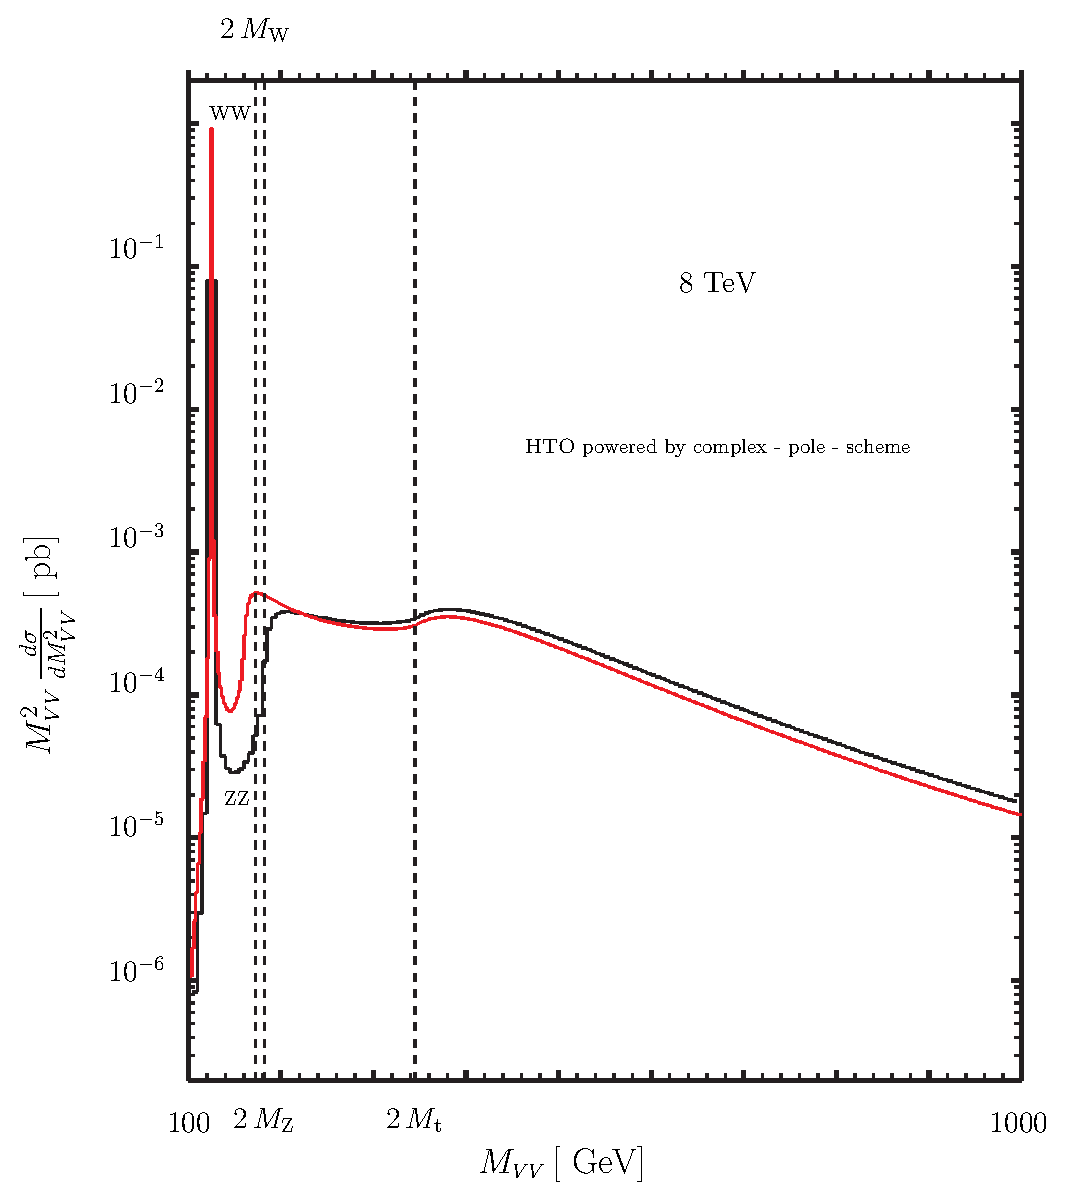
\includegraphics[width=0.46\linewidth]{{LHC_Pheno/lhzwa_fig1b}.eps}
\caption[The NNLO ZZ (black) and WW (red) invariant mass distributions for $m_{H} = \unit{125}{\GeV}$.]{The NNLO ZZ (black) and WW (red) invariant mass distributions for $m_{H} = \unit{125}{\GeV}$\cite{Kauer:2012hd}.}
\label{fig:Higgs_lineshape}
\end{center}
\end{figure}

Following \cite{Caola:2013yja}, we can investigate the total width of the Higgs boson by comparing the on resonance and off resonance cross sections. Generally, the differential cross section of a Higgs boson produced through gluon-gluon fusion decaying into two Z bosons is given by equation \eqref{eq:diff_xsec}. Where $g_{ggH}$ is the effective coupling of the Higgs boson to gluons, $g_{HZZ}$ is the coupling of the Higgs boson to Z bosons, and $\Gamma_{H}$ is the total width of the Higgs boson. Also notice the demarcation of the observed mass of the $4\ell$ system, $m_{4\ell}$, is not necessarily the same as the Higgs boson mass $m_{H}$.

\begin{equation}
\label{eq:diff_xsec}
\frac{d\sigma_{gg \to H \to ZZ}}{d m_{4\ell}} \sim \frac{g_{ggH}^{2}g_{HZZ}^{2}}{\left(m_{4\ell}^{2} - m_{H}^{2}\right)^{2} + m_{H}^{2}\Gamma_{H}^2} 
\end{equation}

When a Higgs boson is produced on the resonance peak $m_{4\ell} \sim m_{H}$ then the mass integral can be evaluated assuming the second term in the denominator will be larger than the first. Giving the on peak cross section in equation \eqref{eq:onpeak_xsec} note that the cross section is proportional to the couplings and inversely the total width of the Higgs boson. However, if a Higgs boson is produced off of the resonance peak, specifically when $m_{4\ell} - m_{H} \gg \Gamma_{H}$, then the cross section becomes independent of the width. Shown in equation \eqref{eq:offpeak_xsec} the off peak cross section becomes proportional to the couplings but the width does not contribute.

\begin{equation}
\label{eq:onpeak_xsec}
\sigma_{gg \to H \to ZZ}^{\text{on peak}} \sim \frac{g_{ggH}^{2}g_{HZZ}^{2}}{\Gamma_{H}} 
\end{equation}

\begin{equation}
\label{eq:offpeak_xsec}
\sigma_{gg \to H \to ZZ}^{\text{off peak}} \sim g_{ggH}^{2}g_{HZZ}^{2} \sim \sigma_{gg \to H \to ZZ}^{\text{on peak}} \times \Gamma_{H}
\end{equation}

From these results we can see that the number of events that are produced on the mass resonance peak is dependent upon the total width of the new boson, while the number of events produced off peak are only dependent upon the couplings to the other SM particles. Thus, as pointed by \cite{Caola:2013yja} measuring the ratio of the on peak and off peak Higgs boson production is equivalent to measuring the total width of the new boson.

Complicating this story, is the quantum mechanical interference between the different $gg \to \ldots \to 4\ell$ processes. While this interference is present for the entire $m_{4\ell}$ range considered in this thesis, at low masses it is a very small and negligible. Above the $2m_{Z}$ mass, the interference between $gg \to ZZ \to 4\ell$ and $gg \to H^{*} \to ZZ \to 4\ell$, figure \ref{fig:gg_??_ZZ_Feyn}, processes needs to be considered. While the off peak signal contribution will scale by $\sigma_{gg \to H \to ZZ}^{\text{on peak}} \times \Gamma_{H}$ the interference between the signal and background term will scale by $\sqrt{\sigma_{gg \to H \to ZZ}^{\text{on peak}} \times \Gamma_{H}}$. 

The impact of these three terms is seen in figure \ref{fig:Higgs_sig/bkg/interf}. Here, one can clearly see the large difference between ignoring (cyan) and correctly accounting (black) for the interference in this region. Neglecting interference one would anticipate a large increase in the yield of the high mass $gg \to \ldots \to ZZ$ contribution, but since the interference between off resonance Higgs boson production and the $gg \to ZZ$ continuum background is destructive, the SM actually predicts that the high mass contribution will be lower than otherwise anticipated.

\begin{figure}
\begin{center}
\includegraphics[width=0.46\linewidth]{{LHC_Pheno/lhzwa_fig2}.eps}
\caption[The LO $ZZ$ invariant mass distribution $gg \to ZZ$ for $m_{H} = \unit{125}{\GeV}$. Black is the total $gg \to \ldots \to ZZ$ contribution once all interfrence effects are taken into account. Red is the $gg \to H^{*} \to ZZ$ signal only, and cyan is the $gg \to \ldots \to ZZ$ contribution ignoring the interference between the two contributions. For scale, the $q\bar{q} \to ZZ$ contribution is shown in blue.]{The LO $ZZ$ invariant mass distribution $gg \to ZZ$ for $m_{H} = \unit{125}{\GeV}$. Black is the total $gg \to \ldots \to ZZ$ contribution once all interfrence effects are taken into account. Red is the $gg \to H^{*} \to ZZ$ signal only, and cyan is the $gg \to \ldots \to ZZ$ contribution ignoring the interference between the two contributions. For scale, the $q\bar{q} \to ZZ$ contribution is shown in blue \cite{Kauer:2012hd}.}
\label{fig:Higgs_sig/bkg/interf}
\end{center}
\end{figure}

\begin{figure}
\begin{center}
\includegraphics[width=0.46\linewidth]{{LHC_Pheno/ZZMass_100-800_SIM_20May2014}.pdf}
\caption[Distribution of the expected four-lepton reconstructed mass in full analysis mass range for the sum of the $4e$, $4\mu$, and $2e2\mu$ channels and for $gg+VV \to ZZ$ processes for a Higgs boson mass of $\unit{125.6}{\GeV}$. The expected distribution for a scenario corresponding to a scaling of the width by 25 is also shown. This illustrates the expected change in $gg+VV \to ZZ$ production when changing the Higgs boson width and at the same time constraining the peak cross section to the SM expectation.]{Distribution of the expected four-lepton reconstructed mass in full analysis mass range for the sum of the $4e$, $4\mu$, and $2e2\mu$ channels and for $gg+VV \to ZZ$ processes for a Higgs boson mass of $\unit{125.6}{\GeV}$. The expected distribution for a scenario corresponding to a scaling of the width by 25 is also shown. This illustrates the expected change in $gg+VV \to ZZ$ production when changing the Higgs boson width and at the same time constraining the peak cross section to the SM expectation \cite{Khachatryan:2014iha}.}
\label{fig:CMS_gg_ZZ}
\end{center}
\end{figure}

The resulting $m_{4\ell}$ distributions for two hypothetical bosons are shown in figure \ref{fig:CMS_gg_ZZ}, they both have the same on peak cross section but different total widths. The result is a change in the total number of events expected in the analysis. Additionally, the shape of the $m_{4\ell}$ distribution and the kinematics of the $4\ell$ will be different. A detailed description of how all of these factors are used to determine the width is given in section \ref{sec:Width_Experiment}. Also included in this image and analysis is the analogous effect for the VBF production mode.

\section{Spin and Parity of a Single-Produced Resonance}
\label{sec:Higgs_Spin_Pheno}

Using the decay rates and kinematics of a newly observed resonance one can piece together the quantum mechanical properties of the original boson. Once a new particle is observed, its spin and parity quantum numbers need to be determined. This will confirm if the new particle is the Higgs boson that was predicted or something entirely, or partially, different. Using the $H \to ZZ \to 4\ell$ decay channel is the best way to study these properties because of the small, well understood background contributions, and because all of the final state particles can be detected by CMS and have excellent precision. 

In basic terms, when a new particle is produced in a collision its spin and parity quantum numbers restrict the allowed types of interactions it can have with SM particles. This feature can be observed by investigating the kinematic distributions of the decay products or the particles produced in association with the new resonance. Of particular interest for this thesis work are the $X \to VV$ couplings (HVV). Where $V$ is any vector boson (Z, W, $\gamma$, g), and $X$ is the new resonance. When this new resonance is spin-0, we will use $H$ because the Higgs boson is predicted to be spin-0. While this vertex can be studied by using the production or decay of a new particle we will focus on the properties that can be determined from the decay products. 

When a new boson is produced it can be either spin-zero, one, or two\footnote{Unless, the resonance is actually two particles with a mass difference less than the experimental resolution.}. In this work each is considered as a possibility for a new resonance, and the differences between their kinematics are used to study and classify the newly observed boson. The relevant phenomenology for these interactions is presented below.

\subsection{Decay of a spin-zero resonance}
\label{sec:Spin0_Pheno}

The scattering amplitude describing the interaction between a spin-zero H boson and two spin-one gauge bosons $VV$ $\left(ZZ, Z\gamma, \gamma\gamma, WW \text{ or } gg\right)$ can be defined as in equation \eqref{eq:formfact-fullampl-spin0}. Where the coupling parameters $a_{i}^{VV}$ can have both real and imaginary parts and in general are form factors which can depend on the suared Lorentz invariant four-momenta of $V_{1}$ and $V_{2}$, $q_{V1}^2$ and $q_{V2}^2$. In this expression, terms of higher order than $q_{V}^2$ have been dropped in the expansion under the assumption that anomalous couplings will only have a small contribution. In this expression, we use a different notation than previous sections and label the field strength tensor of a gauge boson with momentum $q_{Vi}$ and polaraization $\epsilon_{Vi}$ with $f^{\left(i\right) \mu \nu} = \epsilon^{\mu}_{Vi}q_{Vi}^{\nu} - \epsilon^{\nu}_{Vi}q_{Vi}^{\mu}$. ${\tilde f}^{\left(i\right)}_{\mu \nu} = \frac{1}{2}\epsilon_{\mu\nu\rho\sigma}f^{\left(i\right) \rho \sigma}$ is the dual field strength tensor, and the superscript $*$ designates a complex conjugate. The masses of the Z or W boson is labeled as $m_{V1}$, while in the case of massless bosons there is no contribution from this term. To understand the impact form factor will have on the $a_{1}$ term, an energy scale $\Lambda_{1}$ for beyond-SM physics that could impact the SM scattering amplitude is also studied \cite{Anderson:2013afp}. 

\begin{equation}
A(H\to VV) \sim
\left[ a_{1}^{VV}
+ \frac{\kappa_1^{VV}q_{V1}^2 + \kappa_2^{VV} q_{V2}^{2}}{\left(\Lambda_{1}^{VV} \right)^{2}} \right]
m_{V1}^2 \epsilon_{V1}^* \epsilon_{V2}^*
+ a_{2}^{VV}  f_{\mu \nu}^{*(1)}f^{*(2)\mu\nu}
+ a_{3}^{VV}   f^{*(1)}_{\mu \nu} {\tilde f}^{*(2)\mu\nu}
\label{eq:formfact-fullampl-spin0}
\end{equation}

In the SM, the tree-level contribution from $ZZ \left(WW\right)$ correspond to $a_{1}^{ZZ \left(WW\right)} \neq 0$, while the loop-induced SM contribution for $Z\gamma, \gamma\gamma, \text{ and } gg$ is $a_{2}^{VV} \neq 0$. Small SM contributions to the higher order $a_{i}$ terms can come from loop level contributions but, in general, these should be small. Additional restrictions on the allowed values for the $\kappa_{i}$ terms arise from symmetry and gauge invariance. For $ZZ$, they require $\kappa_{1}^{ZZ} = \kappa_{2}^{ZZ} = - \text{exp}\left(-i\phi_{\Lambda1}^{ZZ}\right)$ where $\phi_{\Lambda1}^{ZZ}$ is the relative phase between the $a_{1}^{ZZ}$ and $\Lambda_{1}$ terms. 

The parity conserving contribution from a pseudoscalar particle $\left( 0^{+-}, CP\text{-odd} \right)$ would be generated by the $a_{3}$ term, while a higher order scalar $\left( 0^{++}, CP\text{-even} \right)$ would be generated by $a_{2}$ or $\Lambda_{1}$ contributions. Anomalous contributions for the $\Lambda_{1}, a_{2}, \text{ or } a_{3}$ terms could be a sign of BSM physics and can in general have be complex, allowing for a relative phase between them and the SM $a_{1}$ term. To determine if these anomalous terms contribute to an observed resonance, we parameterize the contribution of one of these terms in an effective cross section fraction. These fractions are given in equation \eqref{eq:fa_definitions}, where $\sigma_{i}$ is the cross section for an $a_{i} = 1, a_{j\neq i} = 0$ particle decaying to the $2e2\mu$ final state\footnote{$\tilde{\sigma}_{\Lambda{1}}$ is the effective cross section of the process corresponding to $\Lambda_{1} = \unit{1}{\TeV}$, given in units of $\femtobarn\cdot\TeV^{4}$.}. The phases $\phi_{ai}$ are used to generalize equation \eqref{eq:formfact-fullampl-spin0} so that the anomalous contributions to be complex.

\begin{equation}\begin{aligned}
f_{\Lambda1} =& \frac{\tilde{\sigma}_{\Lambda1}/\left(\Lambda_{1}\right)^{4}}{\abs{a_1}^2 \sigma_{1} + \abs{a_2}^2 \sigma_{2} + \abs{a_3}^2 \sigma_{3} + \tilde{\sigma}_{\Lambda{1}}/\left(\Lambda_{1}\right)^{4} +\ldots}, &\phi_{\Lambda1}, \\
f_{a2} =& \frac{\abs{a_2}^2 \sigma_{2}}{\abs{a_1}^2 \sigma_{1} + \abs{a_2}^2 \sigma_{2} + \abs{a_3}^2 \sigma_{3} + \tilde{\sigma}_{\Lambda{1}}/\left(\Lambda_{1}\right)^{4} +\ldots}, &\phi_{a2} = \text{arg}\left(\frac{a_{2}}{a_{1}}\right), \\
f_{a3} =& \frac{\abs{a_3}^2 \sigma_{3}}{\abs{a_1}^2 \sigma_{1} + \abs{a_2}^2 \sigma_{2} + \abs{a_3}^2 \sigma_{3} + \tilde{\sigma}_{\Lambda{1}}/\left(\Lambda_{1}\right)^{4} +\ldots}, &\phi_{a3} = \text{arg}\left(\frac{a_{3}}{a_{1}}\right),
\label{eq:fa_definitions}
\end{aligned}\end{equation}


These fractions are especially useful because they allow for great flexibility in the measurements. They are independent of the collider energy so they can be used to compare measurements made at different facilities, they are independent of coupling notation so can be used to translate between many different formulations for the spin-0 interactions, and they are bounded between $0$ and $1$ which allows investigation of the full phase space. 

In CMS studies of these results, analogous fractions are created for the $WW, Z\gamma, \gamma\gamma$ final states. These fractions can be combined for $ZZ$ and $WW$ under different assumptions about the relationships between the $a_{i}^{VV}$ terms. These results were a direct consequence of these studies and are left as a reference for the reader \cite{Khachatryan:2014kca}. 

\subsection{Decay of a spin-one resonance}
\label{sec:Spin1_Pheno}

In the case of a spin-one resonance, the amplitude of its interaction with a pair of massive gauge bosons, ZZ or WW, consists of two independent terms, seen in equation \eqref{eq:ampl-spin1}.

\begin{equation}
A(X_{J=1} \to VV) \sim b_{1}^{VV}  \left[ \left(\epsilon_{V1}^{*}q\right)\left(\epsilon_{V2}^{*}\epsilon_{X}\right) + \left(\epsilon_{V2}^{*}q\right)\left(\epsilon_{V1}^{*}\epsilon_{X}\right) \right] + b_{2}^{VV}  \epsilon_{\alpha\mu\nu\beta}\epsilon_{X}^{\alpha}\epsilon_{V1}^{*\mu}\epsilon_{V2}^{*\nu}{\tilde q}^{\beta}
\label{eq:ampl-spin1}
\end{equation}

Where $\epsilon_{X}$ is the polarization vector of the boson $X$ with spin one, ${q}=q_{V1}+q_{V2}$ and ${\tilde q}=q_{V1}-q_{V2}$~\cite{Gao:2010qx, Bolognesi:2012mm}. Here the $b_{1}^{VV}  \neq 0$ coupling corresponds to a vector particle, while the $b_{2}^{VV} \neq 0$ coupling corresponds to a pseudovector. The $Z\gamma$ interactions of the spin-one particle are not considered, while the $\gamma\gamma$  and $gg$ interactions are forbidden by the Landau-Yang theorem~\cite{Landau:1948kw, Yang:1950rg}, where the $gg$ case is justified by the assumption that the state $X$ is color-neutral.

The evidence for a new boson in the $ZZ$ final state will be presented in section \ref{sec:Search_Results}, similar resonances have been seen in the $H \to \gamma\gamma$ decay channel, preventing the observation from being spin-one \cite{Aad:2012tfa,Chatrchyan:2012ufa,Chatrchyan:2013lba}. In the case that the $ZZ$ resonance is different than the one seen in these references, we test if an observed boson is more consistent with spin-one or the SM predicted Higgs boson. 

Pure vector $\left(1^{+}\right)$, pseudovector $\left(1^{-}\right)$, and mixed vector-pseudovector states are tested using the fraction $f_{b2}^{VV}$ given in equation \eqref{eq:fa_definitions_spin1}. This $f_{b2}^{VV}$ parameter is a continuous unique way to define any state that is a mixture of $1^{+}$ and $1^{-}$. Where $\sigma_{bi}$ is the cross section of the process corresponding to $b_{i} = 1, b_{j\neq i} = 0$ in the $X \to ZZ \to 2e2\mu$ final state.

\begin{equation}
f_{b2}^{VV}  = \frac{\abs{b_{2}^{VV}}^2 \sigma_{b2}}{\abs{b_{1}^{VV}}^2 \sigma_{b1} + \abs{b_{2}^{VV}}^2 \sigma_{b2}},
\label{eq:fa_definitions_spin1}
\end{equation}

\subsection{Decay of a spin-two resonance}
\label{sec:Spin2_Pheno}

In the case of a general spin-two resonance, we test if a new observation is more consistent with the SM Higgs boson or a spin-two boson. The amplitude to describe the $X \to ZZ$ production is given in equation \eqref{eq:ampl-spin2-a} (This same amplitude describes the $gg \to X$ production with $m_{V} = 0$.) where $t^{\mu\nu}$ is the wavefunction of a spin-two particle $X$ given by a symmetric traceless tensor, $m_{V}$ is the mass of the considered gauge boson, and $\Lambda$ is the scale of BSM physics~\cite{Gao:2010qx, Bolognesi:2012mm}. The couplings $c_{1}^{VV}$ and $c_{5}^{VV}$ correspond to the parity-conserving interaction of a spin-two tensor with minimal gravity-like couplings. As in the spin-zero case, the couplings $c_{i}^{VV}$ are in general momentum-dependent form factors. In this analysis it is assumed that the form factors are momentum-independent constants and, thus, only the lowest $q_i^2$  order terms in the scattering amplitude are considered \cite{Khachatryan:2014kca}.



\begin{multline}
\label{eq:ampl-spin2-a}
A(X_{J=2} \to VV)  \sim \Lambda^{-1} \left [
2 c_{1}^{VV} t_{\mu \nu} f^{*1,\mu \alpha} f^{*2,\nu}_{\alpha}
+ 2 c_{2}^{VV} t_{\mu \nu} \frac{q_\alpha q_\beta }{\Lambda^2} f^{*1,\mu \alpha}  f^{*2,\nu \beta}
\right.   \\
\left.
+ c_{3}^{VV} t_{\beta \nu} \frac{{\tilde q}^\beta {\tilde q}^{\alpha}}{\Lambda^2}
 ( f^{*1,\mu \nu} f^{*2}_{\mu \alpha} + f^{*2,\mu \nu} f^{*1}_{\mu \alpha} )
 + c_{ 4}^{VV}t_{\mu \nu} \frac{{\tilde q}^{\nu} {\tilde q}^\mu}{{\Lambda^2} }  f^{*1,\alpha \beta} f^{*2}_{\alpha \beta}
\right.\\
\left. + m_{V}^2  \left (
2 c_{ 5}^{VV}  t_{\mu\nu} \epsilon_{V1}^{*\mu} \epsilon_{V2}^{*\nu}
+2 c_{ 6}^{VV}  t_{\mu \nu} \frac{{\tilde q}^\mu q_\alpha}{\Lambda^2}
\left ( \epsilon_{V1}^{*\nu} \epsilon_{V2}^{*\alpha} -
\epsilon_{V1}^{*\alpha} \epsilon_{V2}^{*\nu} \right )
+c_{ 7}^{VV} t_{\mu \nu}  \frac{{\tilde q}^\mu {\tilde q}^\nu}{\Lambda^2}  \epsilon^*_{V1} \epsilon^*_{V2}
\right)
\right.  \\
\left.
+c_{ 8}^{VV} t_{\mu \nu} \frac{{\tilde q}^{\mu} {\tilde q}^{\nu}}{\Lambda^2}
  f^{*1,\alpha \beta} {\tilde f}^{*2}_{\alpha \beta}
\right.   \\
 \left.
+  m_{V}^2  \left (
c_{ 9}^{VV} t^{\mu \alpha}
\frac{
{\tilde q}_{\alpha} \epsilon_{\mu \nu \rho \sigma} \epsilon_{V1}^{*\nu} \epsilon_{V2}^{*\rho} q^{\sigma}
}{\Lambda^2}
+c_{ 10}^{VV} t^{\mu \alpha}
\frac{
{\tilde q}_{\alpha} \epsilon_{\mu \nu \rho \sigma} q^\rho {\tilde q}^{\sigma}
\left ( \epsilon_{V1}^{*\nu}(q\epsilon_{V2}^*)+
\epsilon_{V2}^{*\nu}(q\epsilon_{V1}^*) \right )
}{\Lambda^4}
\right )
\right ],
\end{multline}


In this work, we study the ten spin-two scenarios listed in table \ref{tab:scenarios}, under the assumption that the production is via gluon-gluon fusion, $q\bar{q}$ production, or without any assumption about the production mechanism. The $2_m^+$ represents a massive graviton-like boson as suggested in models with warped extra dimensions \cite{Randall:1999vf, Randall:1999ee}. A modified minimal coupling model $2^+_{b}$ is also considered, where the SM fields are allowed to propagate in the bulk of the extra dimensions \cite{Agashe:2007zd}, corresponding to $c_1^{VV} << c_5^{VV}$. Additionally eight spin-two models with higher dimension operators are considered \cite{Khachatryan:2014kca}.

\begin{table*}[htbp]
\caption[List of spin-two models with the decay couplings of an exotic $X$ particle. The subscripts $m$ (minimal couplings), $h$ (couplings with higher-dimension operators),
and $b$ (bulk) distinguish different scenarios.]{ List of spin-two models with the decay couplings of an exotic $X$ particle. The subscripts $m$ (minimal couplings), $h$ (couplings with higher-dimension operators), and $b$ (bulk) distinguish different scenarios \cite{Khachatryan:2014kca}. }
\centering
\begin{tabular}{cc}
$J^P$ Model  & $X\to VV$ Couplings \\

\hline

$2_m^+$  &   $c_{ 1}^{VV}=c_{ 5}^{VV}\ne0$     \\

$2_{h2}^+$      &   $c_{ 2}^{VV}\ne0$  \\

$2_{h3}^+$     &   $c_{ 3}^{VV}\ne0$  \\

$2_h^+$  &   $c_{ 4}^{VV}\ne0$  \\

$2_b^+$   &   $c_{ 1}^{VV} << c_{ 5}^{VV}\ne0$ \\

$2_{h6}^+$  &    $c_{ 6}^{VV}\ne0$  \\

$2_{h7}^+$ &   $c_{ 7}^{VV}\ne0$ \\

$2_h^-$  &     $c_{ 8}^{VV}\ne0$  \\

$2_{h9}^-$ &   $c_{ 9}^{VV}\ne0$ \\

$2_{h10}^-$ &  $c_{ 10}^{VV}\ne0$ \\
\end{tabular}

\label{tab:scenarios}
\end{table*}
